\documentclass{article}
\usepackage{caption}
\usepackage{subcaption}
\usepackage{graphicx}
\usepackage{tikz}
\usepackage{tikzsymbols}
\usetikzlibrary{calc,patterns,shapes.geometric}
\usepackage{float}
\usepackage{pdflscape}
\usepackage{geometry}


\def\centerarc[#1](#2)(#3:#4:#5){\draw[#1] ($(#2)+({#5*cos(#3)},{#5*sin(#3)})$) arc (#3:#4:#5);}

\pagestyle{empty}
\begin{document}
	\centering
	\begin{figure}[H]
		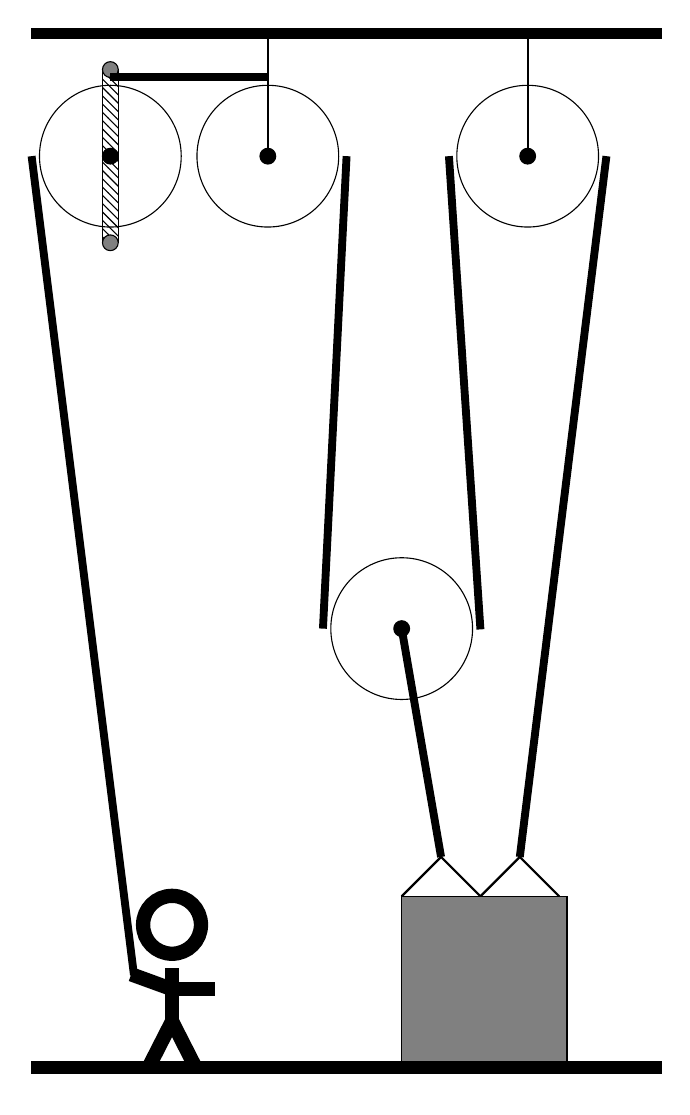
\begin{tikzpicture}
			%%%%% START %%%%%
			\def\a{10}
			\def\radlg{\radrp-0.1}
			\def\radrp{1}
			\def\radsm{0.1}
			\def\xone{1}
			\def\yone{\a-0.15*\a}
			\def\xtwo{\xone+3.3}
			\def\ytwo{\a-0.15*\a}
			\def\xthree{\xone+1.7}
			\def\ythree{\a-0.75*\a}
			\def\xh{3.2}
			\def\hlentwo{\yone+0.26*\a}
			\def\hlen{\yone+0.26*\a}
			\def\width{1mm}
			\def\ywallone{\yone}
			\def\xwallone{\xone-2}
			\def\bump{0.1}
			
			\draw[fill=black] (-2,\a) rectangle (6,\a+0.125);
			
			\draw (\xone,\yone) circle (\radlg);
			\draw[fill=black] (\xone,\yone) circle (\radsm);
			\draw[thick] (\xone,\yone) -- (\xone,\a);
			
			\draw (\xtwo,\ytwo) circle (\radlg);
			\draw[fill=black] (\xtwo,\ytwo) circle (\radsm);
			\draw[thick] (\xtwo,\ytwo) -- (\xtwo,\a);
			
			\draw (\xthree,\ythree) circle (\radlg);
			\draw[fill=black] (\xthree,\ythree) circle (\radsm);
			
			
			\draw[thick]  (\xh-0.5,\ytwo-\hlentwo-0.5) -- (\xh,\ytwo-\hlentwo) -- (\xh+0.5,\ytwo-\hlentwo-0.5);
			\draw[thick]  (\xh+0.5,\yone-\hlen-0.5) -- (\xh+1,\yone-\hlen) -- (\xh+1.5,\yone-\hlen-0.5);
			\draw[fill=black!50] (\xh-0.5,\yone-\hlen-0.5) rectangle (\xh+1.6,\yone-\hlen-0.5-2.1);
			
			%first extra polly
			\draw (\xwallone,\ywallone) circle (\radlg);
			\draw[fill=black] (\xwallone,\ywallone) circle (\radsm);
			\draw[pattern=north west lines, pattern color=black] (\xwallone-0.1,\ywallone+\radrp+\bump) rectangle (\xwallone+0.1,\ywallone-\radrp-\bump); 
			\draw[fill=black!50] (\xwallone,\ywallone+\radrp+\bump) circle (\radsm);
			\draw[fill=black!50] (\xwallone,\ywallone-\radrp-\bump) circle (\radsm);
			
			

			
			
			\draw[line width=\width](-0.7,-1.9) -- 	 (\xwallone-\radrp, \ywallone);
			\centerarc[line width=\width](\xwallone,\ywallone)(90:180:\radrp);
			
			\draw[line width=\width](\xwallone, \ywallone+\radrp) -- (\xone,\yone+\radrp);
			\centerarc[line width=\width](\xone,\yone)(0:90:\radrp);
			\draw[line width=\width](\xone+\radrp,\yone) -- (\xthree-\radrp,\ythree);
			\centerarc[line width=\width](\xthree,\ythree)(180:370:\radrp);
			\draw[line width=\width] (\xthree+\radrp,\ythree-0.01) -- (\xtwo-\radrp,\ytwo);
			\centerarc[line width=\width](\xtwo,\ytwo)(0:180:\radrp);
			\draw[line width=\width](\xh+1,\yone-\hlen) -- (\xtwo+\radrp,\ytwo);
			\draw[line width=\width] (\xh,\yone-\hlen) -- (\xthree,\ythree);
			
			\node at (-0.2,-2) {\Strichmaxerl[10][-20][0]};
			
			\draw[fill=black] (-2,-3) rectangle (6,-3.15);
			%%%%% START %%%%%
		\end{tikzpicture}
	\end{figure}
	
\end{document}